\section{Problem 1}
\textit{ Modify the Matlab code to have a second excitation phase delayed . Study the gain pattern of the two dipoles resonating at 850 MHz as a function of distance between the dipoles and the phase difference between their excitation. Compare the numerical results with the theoretical results from section 6.2 from Balanis’ Antenna Theory second edition.}\\

First the simulation environment is setup in section \ref{sec:mm7pb1_simulation} with two sources. Because the afc program can't handle two sources by itself the code needs to be changed and one of the sources is consisting of a resistor instead of a source. The change to the code is explained in section \ref{sec:mm7pb1_implementation}. In section \ref{sec:mm7pb1_results} the result are discussed and compared to the theory. 


\subsection{Setting up the simulation environment}\label{sec:mm7pb1_simulation}
Two dipole antennas is simulated in the AFC program to study the gain pattern as a function of the distance between the dipoles and the phase difference. The parameters for the setup of the two dipoles in the simulation environment is shown in table \ref{tab1:ap_mm7_pb1} and the simulation geometry is shown in figure \ref{fig1:ap_mm7_pb1}. 

\ptable{| p{12cm} | p{6cm} |}{ %
Parameter 		&	Value 			\\ \hline
Dipole size 		        &	$18 cells$	$\approx$ 176mm        \\ \hline
Resistor size 50 $\Omega$ (Fake dipole)     &	$18 cells$	$\approx$ 176mm        \\ \hline
Dipole position (x axis) 		        &	$50 cells$	        \\ \hline
Cell size 		        &	$\SI{0.01}{\meter}$	        \\ \hline
Excitation lower freq 		        &	$\SI{1}{\hertz}$	        \\ \hline
Excitation higher freq 		        &	$\SI{1.7}{\giga\hertz}$	        \\ \hline
}{Simulation and design parameters}{tab1:ap_mm7_pb1}

The placement of the resistor depend on the distance between the two sources. In figure \ref{fig1:ap_mm7_pb1} an example is shown with a distance between the two sources of $\approx$8 cm. 

\begin{figure}[!h]
  \centering
  \includegraphics[width=12cm]{figures/geometry_two_dipoles.eps}
  \caption{Plot showing the two dipoles plotted, one with a source and the other with a resistor}
  \label{fig1:ap_mm7_pb1}
\end{figure}


\subsection{Implementation to the AFC code}\label{sec:mm7pb1_implementation}
To calculate the time difference used in the code the following formulas is used. The time spacing,$\Delta t$, in the program is controlled in the advanced FDTD settings, by equation \ref{eq1:mm7_prob1}.
\begin{flalign}
&& \Delta t =& \frac{\Delta x}{c \sqrt{3}} \cdot 0.999 & \label{eq1:mm7_prob1}
\end{flalign} 
$\Delta x$ is the cell size, and with a cell size of 0.01 [m] the $\Delta t$ becomes 
\begin{flalign}\label{eq1:mm7_prob1}
&& \Delta t =& \frac{0.01}{3E8 \sqrt{3}} \cdot 0.999 & \\
&& \approx & 1.92E-11 & 
\end{flalign} 

The time spacing between the two sources can be determined from the distance between them by taking the ratio of the distance the wave needs to travel and the wavelength. 
\begin{flalign}
&& d =&K \cdot lambda & \\
&& K =& \frac{d}{lambda} &
\end{flalign}
The time it takes to travel the distance can then be found from 
\begin{flalign}
&& \tau =& K \cdot \frac{1}{f_{0}} &
\end{flalign}

To translate this into the index, t, used in the code.
\begin{flalign}
 && t0 =& \frac{\tau}{\Delta t} &
\end{flalign}

The code that needs to be modified is in the function MatlabFDTD in the afc.m file. Under the resistive source an update to the electric field is added, the change is depending on how the two sources is oriented. For the settings explained in section \ref{sec:mm7pb1_simulation} the updates needs to be done in the Ez, and can be seen in the code snippet \ref{cl:afc}.  
\code{language=Matlab,caption = AFC program,label=cl:afc,linerange={6906-6912},firstnumber=6887}{code/mm6/afc/afc2.m}


\subsection{Results}
In \citep{lit:AT} chapter 6 array structure is described. For a two element array it applies that if the antennas is placed with a distance of $d=\frac{\lambda}{4}$ between each other the phase difference between them will chancel in one direction and add in the other \citep[Sec. 6.2]{lit:AT}. This has been simulated an the result is shown in a 3d plot in figure \ref{fig2:ap_mm7_pb1} and a 2d plot for the X-Y plane in figure \ref{fig3:ap_mm7_pb1}. As can be seen in the two plots the two antennas creates a directional antenna.

\begin{figure}[!h]
  \centering
  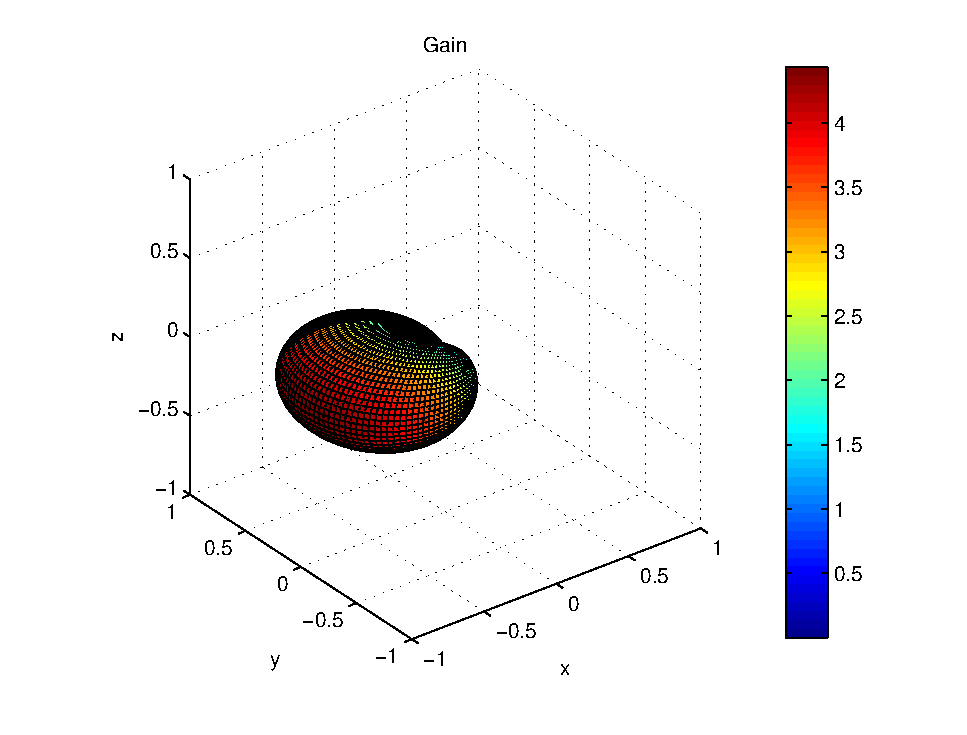
\includegraphics[width=11cm]{figures/two_dipoles_lambda_4.eps}
  \caption{3D-Plot showing the directional properties when the dipoles have a distance of $\frac{\lambda}{4}$}
  \label{fig2:ap_mm7_pb1}
\end{figure}
\begin{figure}[!h]
  \centering
  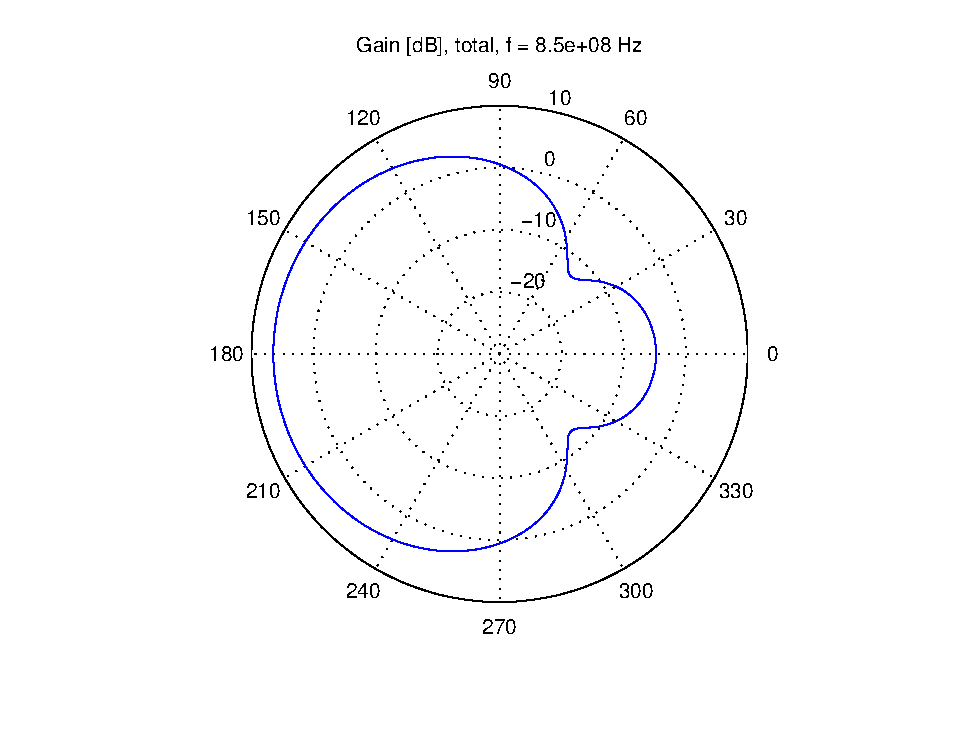
\includegraphics[width=11cm]{figures/two_dipoles_lambda_4_xyplot.eps}
  \caption{2D-Plot showing the directional properties when the dipoles have a distance of $\frac{\lambda}{4}$}
  \label{fig3:ap_mm7_pb1}
\end{figure}

If the two antennas is placed with a distance of $d=\frac{\lambda}{2}$ the two array should create what is called end-fire \citep[Sec. 6.3.2]{lit:AT}. This has also been simulated and the result can be seen in the 3d-plot in figure \ref{fig4:ap_mm7_pb1} and a 2d plot for the X-Y plane in figure \ref{fig5:ap_mm7_pb1}.

\begin{figure}[!h]
  \centering
  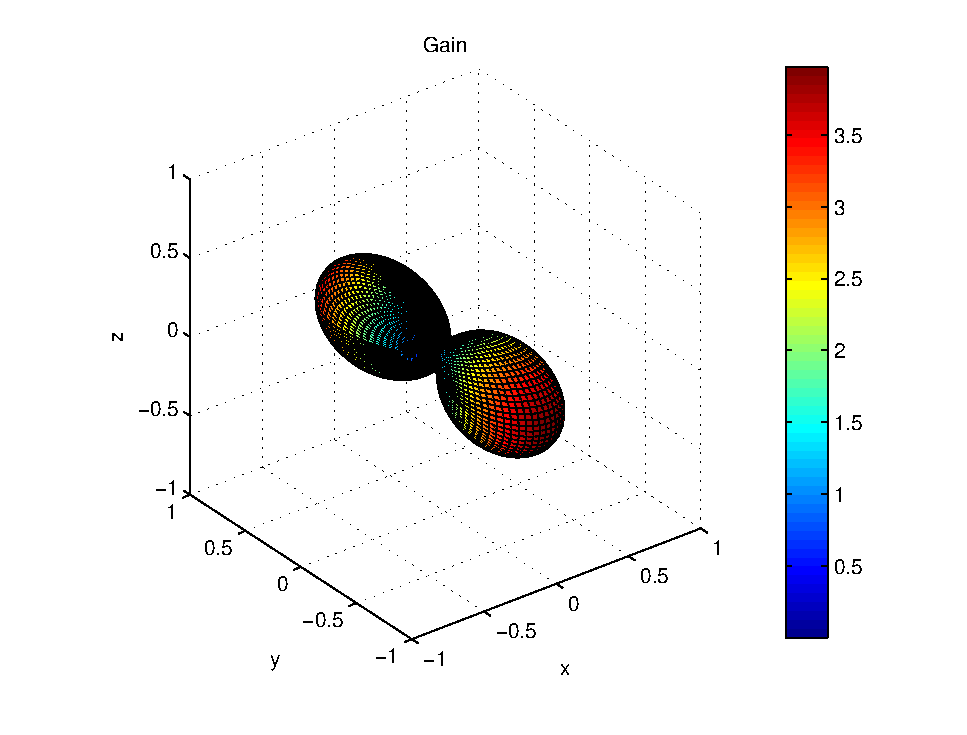
\includegraphics[width=11cm]{figures/two_dipoles_lambda_2.eps}
  \caption{3D-Plot showing the directional properties when the dipoles have a distance of $\frac{\lambda}{2}$}
  \label{fig4:ap_mm7_pb1}
\end{figure}
\begin{figure}[!h]
  \centering
  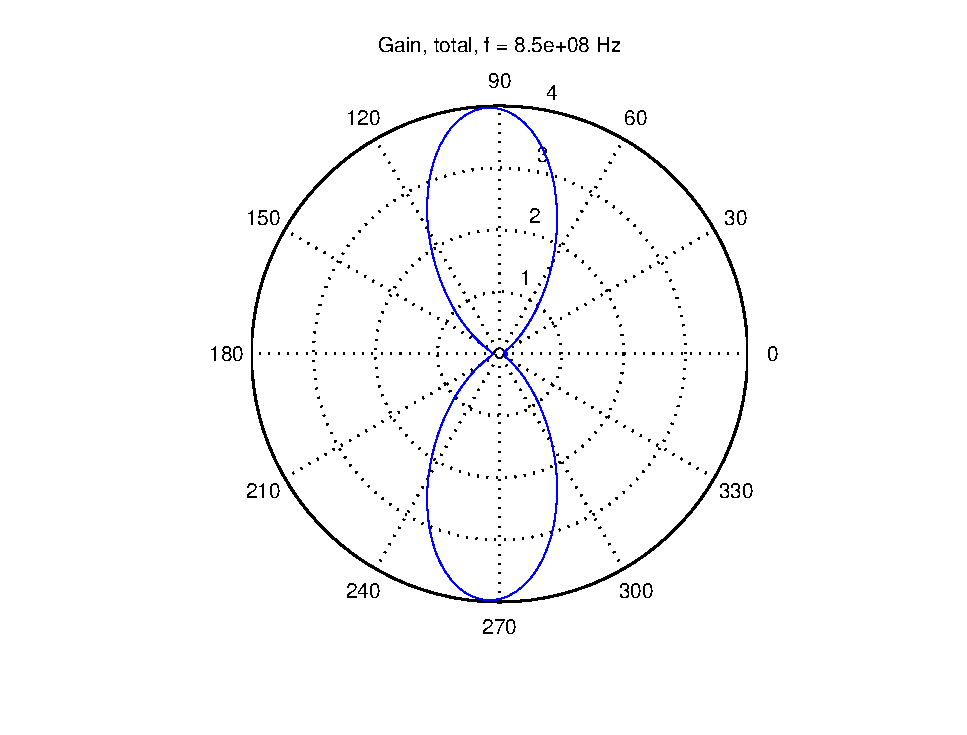
\includegraphics[width=11cm]{figures/two_dipoles_lambda_2_xyplot.eps}
  \caption{2D-Plot showing the directional properties when the dipoles have a distance of $\frac{\lambda}{2}$}
  \label{fig5:ap_mm7_pb1}
\end{figure}